\documentclass[11pt,a4paper]{article}
\usepackage{gtu-el-yazisi}
\begin{document}
\notbilgi{Elektronik II}{Frekans cevabı: alçak/yüksek frekans, Miller teoremi}{Ders9.pdf}

\sayfa{1}
\section{BJT}
\begin{gather*}
g_m = \frac{I_C}{V_T} \\
r_e = 1/g_m \\
r_\pi = (\beta+1)\,r_e
\end{gather*}

\section{Mosfet}
\begin{gather*}
g_m = \frac{2 I_D}{V_{OV}} \\
r_o = \frac{|V_A|}{I_{C,D}}
\end{gather*}
\textit{(BJT bloğundaki $r_\pi$ satırından MOSFET bloğundaki $r_o$ satırına bir çizgi çekilmiş.)}

\begin{gather*}
I_D = \tfrac12\,\mu_n C_{ox}\,\frac{W}{L}\,(V_{GS}-V_t)^2\,(1+\lambda V_{DS}) \\
I_C = I_S\, e^{\frac{V_{BE}}{V_T}}
\end{gather*}

\[ f_L = \frac{1}{2\pi}\left(\underbrace{\frac{1}{R_1 C_1}}_{10} + \underbrace{\frac{1}{R_2 C_2}}_{\substack{50\,\okunamadi{Hz}\\ \Downarrow\\ \text{dominant}}} + \underbrace{\frac{1}{R_3 C_3}}_{100}\right) \]

\sekilnotu[1]{Eşdeğer direnç şeması: solda toprağa bağlı $R_1$; iki açık uç (``o'' ``o'', kondansatörün olduğu yer) arasında çift yönlü ok ve üstünde ``$R_{eq}$''; sağdaki uçtan çıkan ortak düğümden toprağa bağlı $R_2$ ve $R_3$ (paralel).}

\[ R_{eq} = R_1 + R_2 \parallel R_3 \]

\section{The CE amplifier}
\sekilnotu[1]{Ortak emiter (CE) yükselteç devresi, NPN BJT. Üstte $V_{CC}$ (yukarı ok) ve $R_C$ ile kolektör; kolektörden $C_{C2}$ kuplaj kondansatörü ile toprağa bağlı $R_L$ yük direncine ve $v_O$ çıkışına. Giriş: $V_{sig}$ kaynağı (toprağa bağlı), $R_{sig}$ ve (etiketsiz) kuplaj kondansatörü üzerinden base'e. Emiter: $C_E$ bypass kondansatörü ile toprağa ve aşağı yönlü $I$ akım kaynağı ile $-V_{EE}$'ye bağlı. Aynı devre sağda turkuaz kalemle ikinci kez çizilmiş.}

\sekilnotu[1]{Küçük işaret eşdeğer devresi: $R_{sig}$, ardından turuncu kalemle işaretlenmiş $C_{C1}$ kondansatörü; sonraki düğümden toprağa $R_B$; aynı düğümden $r_\pi$ (üzerinde $v_\pi$, ``$+$'' ve ``$-$'' işaretli) ve bağımlı akım kaynağı $g_m v_\pi$; kaynağın sağında toprağa bağlı $R_C$ ve $R_L$, ikisinin üstünde turuncu/turkuaz kalemle işaretlenmiş $C_{C2}$; alt düğümde (emiter) kırmızı kalemle işaretlenmiş $C_E$ kondansatörü (toprağa).}

\[ R_{CC1} = R_{sig} + R_B \parallel r_\pi \]

\[ R_{E1} = \frac{R_{sig} \parallel R_B + r_\pi}{\beta+1} = r_e + \frac{R_{sig} \parallel R_B}{\beta+1} \]

\[ f_L = \frac{1}{2\pi}\left[\frac{1}{R_{CC1}\,C_{C1}} + \frac{1}{R_{CC2}\,C_{C2}} + \frac{1}{R_{E1}\,C_E}\right] \]

\sayfa{2}
\[ R_{CC2} = R_C + R_L \]

\section{Soru}
\sekilnotu[2]{Ortak base (CB) yükselteç devresi: NPN BJT, base solda toprağa bağlı; kolektör üstte $R_C$ ile $V_{DD}$'ye bağlı, ayrıca $C_{C2}$ kuplaj kondansatörü ile toprağa bağlı $R_L$'ye ve çıkışa; emiter: aşağı yönlü bir $I$ akım kaynağına ve $C_{C1}$ kuplaj kondansatörü ile toprağa bağlı $v_{sig}$ kaynağına bağlı.}

\[ f_L = \ ? \]

\sekilnotu[2]{Küçük işaret eşdeğer devresi: solda toprağa bağlı uçtan $r_\pi$ (üzerinde $v_\pi$, ``$+$'' ve ``$-$'' işaretli), alt düğümü ``E'' olarak işaretli; bağımlı akım kaynağı $g_m v_\pi$ ($r_\pi$ ve kaynak turuncu kesikli çerçeve içinde). E düğümünden aşağı $C_{C1}$ kondansatörü ve toprağa bağlı $v_{sig}$ kaynağı (turuncu kalemle işaretli). Sağda ``C'' düğümü: toprağa bağlı $R_C$ ve $C_{C2}$ üzerinden toprağa bağlı $R_L$ ($C_{C2}$ turuncu kalemle işaretli).}

\noindent from $C_{C1}$ \qquad $R_{CC1} \approx r_e$

\noindent from $C_{C2}$ \qquad $R_{CC2} = R_C + R_L$

\begin{center}
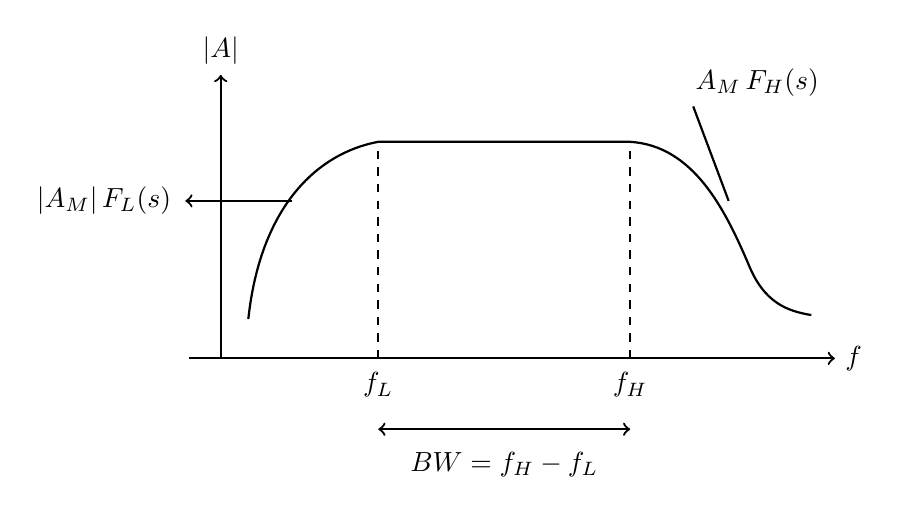
\begin{tikzpicture}[line width=0.8pt]
  \draw[->] (-0.4,0) -- (7.8,0) node[right] {$f$};
  \draw[->] (0,0) -- (0,3.6) node[above] {$|A|$};
  \draw (0.35,0.5) .. controls (0.5,1.9) and (1.2,2.6) .. (2.0,2.75) -- (5.2,2.75)
        .. controls (6.0,2.7) and (6.4,1.9) .. (6.7,1.2) .. controls (6.9,0.7) and (7.2,0.6) .. (7.5,0.55);
  \draw[dashed] (2.0,0) -- (2.0,2.75);
  \draw[dashed] (5.2,0) -- (5.2,2.75);
  \node[below] at (2.0,-0.05) {$f_L$};
  \node[below] at (5.2,-0.05) {$f_H$};
  \draw[<->] (2.0,-0.9) -- (5.2,-0.9);
  \node at (3.6,-1.35) {$BW = f_H - f_L$};
  \node[anchor=east] at (-0.5,2.0) {$|A_M|\,F_L(s)$};
  \draw[->] (0.9,2.0) -- (-0.45,2.0);
  \node[anchor=south west] at (5.9,3.2) {$A_M\,F_H(s)$};
  \draw (6.0,3.2) -- (6.45,2.0);
\end{tikzpicture}
\end{center}

\sayfa{3}
\sekilnotu[3]{NMOS kesit çizimi: ortada ``p-sub'' etiketli taban; üstte solda ``S'' (source) ve sağda ``D'' (drain) uçlarına çıkan oklar, altlarında iki n$^+$ bölgesi; ikisinin arasında gate (altında kesikli kanal çizgisi, üstünde ``$C_{ox}$'' benzeri bir etiket). Source ve drain bölgelerinin altından, kırmızı kalemle, tabana (toprağa) giden birer ters yönlü diyot (kavşak kapasitesi) ve yanlarında küçük kondansatör işaretleri çizilmiş.}

\[ \textcolor{kirmizikalem}{\text{Triode Region:}}\quad C_{gs} = C_{gd} = \frac{1}{2}\,W L\,C_{ox} \]

\[ \textcolor{kirmizikalem}{\text{Sat region :}}\quad \begin{cases} C_{gs} = \dfrac{2}{3}\,W L\,C_{ox} \\[2mm] C_{gd} = 0 \end{cases} \]

\[ \textcolor{kirmizikalem}{\text{cut off region:}}\quad \begin{cases} C_{gs} = C_{gd} = 0 \\ C_{gb} = W L\,C_{ox} \end{cases} \]

\[ \textcolor{kirmizikalem}{\text{overlap capacitance:}}\quad C_{ov} = W L_{ov}\,C_{ox} \]

\[ {\color{turuncukalem}\uparrow}\ I_D = \frac{1}{2}\,\mu_n C_{ox}\,\overset{\color{turuncukalem}\uparrow}{\frac{W}{L}}\,(V_{GS}-V_t)^2 \]

\begin{align*}
|A_0| &= g_m r_o \\
      &= \frac{2 I_D}{V_{OV}} \cdot \frac{V_A'\,L}{I_D} \\
      &= \frac{2\cdot V_A'\,L\,{\color{turuncukalem}\uparrow}}{V_{OV}\ {\color{turuncukalem}\rightarrow}}
\end{align*}

\begin{center}
\begin{tikzpicture}[line width=0.8pt]
  \draw[->] (0,0) -- (7.5,0) node[right] {$f$};
  \draw[->] (0,0) -- (0,4.9) node[above] {$|A|$};
  \draw (0,0) .. controls (0.6,0.1) and (1.0,2.2) .. (1.7,2.8) -- (5.8,2.8)
        .. controls (6.1,2.75) and (6.2,1.0) .. (6.5,0);
  \draw[kirmizikalem] (0.1,0) .. controls (1.2,0.2) and (2.0,4.5) .. (3.7,4.5)
        .. controls (4.5,4.5) and (4.5,1.6) .. (5.2,0.8) .. controls (5.6,0.3) and (6.0,0.05) .. (6.7,0);
  \draw[turuncukalem] (0,0) -- (0.5,0.1) .. controls (0.6,1.0) and (0.7,1.6) .. (0.8,1.65) -- (7.0,1.5)
        -- (7.1,0.9) .. controls (7.2,0.5) and (7.6,0.3) .. (8.0,0.1);
  \draw[dashed] (1.7,0) -- (1.7,2.8);
  \draw[dashed] (5.8,0) -- (5.8,2.8);
  \node[below] at (1.7,-0.05) {$f_L$};
  \node[below] at (5.8,-0.05) {$f_H$};
  \draw[<->] (1.7,-0.9) -- (5.8,-0.9);
  \node at (3.75,-1.35) {$BW = f_H - f_L$};
\end{tikzpicture}
\end{center}

\noindent Source body capacitance:
\[ C_{sb} = \frac{C_{sb0}}{\sqrt{1+\dfrac{V_{SB}}{V_0}}} \]

\[ C_{db} = \frac{C_{db0}}{\sqrt{1+\dfrac{V_{DB}}{V_0}}} \]

\sayfa{4}
\sekilnotu[4]{Ortak source MOSFET yükselteci: $V_{DD}$ (yukarı ok) --- $R_D$ --- drain düğümü; drain düğümünden doğrudan toprağa bağlı $R_L$ (kuplaj kondansatörü yok); source toprağa bağlı; gate, $R_{sig}$ üzerinden toprağa bağlı $v_{sig}$ kaynağına bağlı.}

\sekilnotu[4]{Küçük işaret eşdeğer devresi: $v_{sig}$ (toprağa bağlı) --- $R_{sig}$ --- gate ucu (``$+$''); source ucu (``$-$''); aralarında $V_{gs}$ ve kırmızı kalemle $C_{gs}$. Gate ucundan çıkış düğümüne kırmızı kalemle çizilmiş $C_{gd}$ kondansatörü; yanında turuncu okla ``bir feedback neden oluyor''. Bağımlı akım kaynağı $g_m V_{gs}$; çıkış düğümünden toprağa $r_o$, $R_D$, $R_L$ ve kırmızı kalemle $C_{db}$; çıkış $V_{out}$.}

\noindent Analiz yaparken açık devre yapılırlar

\sekilnotu[4]{Kondansatörlerin açık devre yapıldığı eşdeğer devre: soldan toprağa bağlı $R_{sig}$, ardından gate ucu (``$+$'') ve source ucu (``$-$''), $V_{gs}$; bu iki uç arasında turuncu/kırmızı kalemle çizilmiş iki ok. Bağımlı akım kaynağı $g_m V_{gs}$; çıkış düğümünden toprağa $r_o$, $R_D$, $R_L$; $V_{out}$ hattı kırmızı ile işaretli.}

\formulkutu{R_{gs} = R_{sig} \parallel}
\textit{(ifade bu şekilde yarım bırakılmış)}

\sekilnotu[4]{Test devresi: $R_{sig}$ altında turuncu bir ok; gate ucu ile çıkış (drain) düğümü arasında kırmızı kalemle bir $V_x$ test kaynağı (daire; gate tarafı ``$-$'', drain tarafı ``$+$'') ve $I_x$ akımı; düğümde turuncu oklar: ``$I_x$'' (sağa) ve ``$g_m V_{gs}$'' (sola). Bağımlı akım kaynağı $g_m V_{gs}$; çıkışta toprağa bağlı $R_L' = r_o \parallel R_D \parallel R_L$; $V_{out}$ hattı ve $C_{db}$ kırmızı kalemle işaretli.}

\[ \frac{V_x}{I_x} = \ ? \]

\begin{align*}
V_{out} = V_x + V_{gs} &= (I_x - g_m V_{gs})\,R_L' \\
V_{gs} &= -R_{sig}\, I_x \\
V_x - R_{sig}\, I_x &= (I_x + g_m R_{sig}\, I_x)\,R_L'
\end{align*}
\textit{(Aynı denklemler sağ tarafa turuncu kalemle tekrar yazılmış; son satırda $g_m$ ile $I_x$ arasına ok işaretiyle ``$R_{sig}$'' eklenmiş.)}

\sayfa{5}
\[ V_x = I_x\left(R_{sig}\,(1+g_m R_L') + R_L'\right) \]

\[ \frac{V_x}{I_x} = R_{sig}\,(1+g_m R_L') + R_L' \]

\formulkutu{R_{gd} = R_{sig}\,(1+g_m R_L') + R_L'}
\formulkutu{R_{db} = R_L'}
\textit{(Bu dört satır sağ tarafa turuncu kalemle bir kez daha yazılmış: $V_x/I_x = R_{gd}$ ve $R_{db} = R_L'$.)}

\[ \tau = RC \]

\[ \tau_H = R_{gs}\,C_{gs} + R_{gd}\,C_{gd} + R_{db}\,C_{db} \]

\[ f_H = \frac{1}{2\pi\,\tau_H} \]

\[ \textcolor{kirmizikalem}{\text{unity gain frequency :}}\quad f_T = \frac{g_m}{2\pi\,(C_{gs}+C_{gd})} \]
\textit{(Aynı formül sağ tarafa turuncu kalemle tekrar yazılmış.)}

\begin{center}
\begin{tikzpicture}[line width=0.8pt]
  \draw[->] (-0.2,0) -- (6.2,0);
  \draw[->] (0,-1.0) -- (0,3.0);
  \node[turuncukalem,anchor=south west] at (0.3,2.75) {$|\mathrm{dB}|$};
  \draw (0,0) .. controls (0.5,0.1) and (0.8,1.6) .. (1.2,1.7) -- (3.9,1.8)
        .. controls (4.3,1.7) and (4.3,0.4) .. (4.8,0.15) .. controls (5.2,-0.1) and (5.6,-0.1) .. (6.0,0.05);
  \fill[turuncukalem] (5.0,0) circle (1.5pt);
  \draw[->,turuncukalem] (5.0,0) -- (5.0,-0.45);
  \node[turuncukalem,below] at (5.0,-0.45) {$f_T$};
  \node[turuncukalem,anchor=west,align=left] at (5.5,-0.55) {x ile kesiştiği\\ nokta};
  \node[turuncukalem,anchor=west,align=left] at (4.3,2.5) {gain'i 1 olan\\ nokta};
\end{tikzpicture}
\end{center}

\sekilnotu[5]{Yapıştırılmış basılı şekil (``Model''): MOSFET yüksek frekans küçük işaret eşdeğer devresi (mavi zeminli). G ucundan $C_{gd}$ ile D ucuna; gate düğümünden $C_{gs}$ ($V_{gs}$ ``$+$'' üstte, ``$-$'' altta) ile source düğümüne; bağımlı kaynaklar $g_m V_{gs}$ ve $g_{mb}V_{bs}$, $r_o$; source ile gövde (B) arasında $C_{sb}$ ($V_{bs}$), drain ile gövde arasında $C_{db}$; S ve B uçları altta. Üzerine siyah kalemle, $g_{mb}V_{bs}$ kaynağının üstünden ve $C_{db}$ kondansatörünün üstünden birer çizgi çekilmiş.}

\section{In BJT}
\[ C_\mu\footnotemark = \frac{C_{\mu 0}}{\left(1+\dfrac{V_{CB}}{V_{0c}}\right)^{m}} \]
\footnotetext{Claude notu: Alt indis el yazısında ``n'' gibi okunuyor; $V_{CB}$ içerdiği için $\mu$ (CB eklemi) seçildi.}

\sayfa{6}
\sekilnotu[6]{Yapıştırılmış basılı şekil: BJT hibrit-$\pi$ yüksek frekans modeli (mavi zeminli). B ucundan $r_x$ ile B' düğümüne; B' ile E arasında $r_\pi$ ($V_\pi$, ``$+$'' üstte) ve $C_\pi$; B' ile C arasında $C_\mu$; C ile E arasında $g_m V_\pi$ bağımlı kaynağı ve $r_o$; uçlar B, C ve E.}

\sekilnotu[6]{CE yükselteç devresi (NPN BJT, elle çizilmiş): üstte $V_{CC}$ (yukarı ok) ve $R_C$ ile kolektör; kolektörden $C_{C2}$ ile toprağa bağlı $R_L$ yük direncine; giriş: $v_{sig}$ (toprağa bağlı), $R_{sig}$ ve (etiketsiz) kuplaj kondansatörü ile base'e; emiter: aşağı yönlü bir akım kaynağı ve toprağa bağlı $C_{C3}$ kondansatörü.}

\sekilnotu[6]{Yüksek frekans küçük işaret eşdeğer devresi: $v_{sig}$ (turuncu kalemle işaretli, toprağa bağlı) --- $R_{sig}$ --- B' düğümü; B' ile alt (toprak) hattı arasında $r_\pi$ ($v_\pi$, ``$+$'' üstte ``$-$'' altta) ve turuncu kalemle işaretlenmiş $C_\pi$; B' ile çıkış düğümü arasında çift çizgi ve oklarla çizilmiş $C_\mu$; bağımlı akım kaynağı $g_m v_\pi$; çıkış düğümü ``C'' olarak işaretli, ona bağlı iki direnç $R_C$ ve $R_L$ (toprağa).}

\[ R_{C\pi} = R_{sig} \]

\sekilnotu[6]{Turuncu kalemle çizilmiş test devresi: solda toprağa bağlı $R_{sig}$ ve $r_\pi$ (paralel); bunların üst düğümü ile sağdaki düğüm arasında $I_x$ test akım kaynağı (daire içinde ok) ve $V_x$ (``$+$'' solda, ``$-$'' sağda); sağ düğümden toprağa bağlı $g_m v_\pi$ bağımlı kaynağı, $R_C$ ve $R_L$; üstte ``$R_C \parallel R_L$'' notu.}

\noindent Short circuit collector current

\sayfa{7}
\sekilnotu[7]{Basılı materyal (ders kitabı, Şekil 9.10): $|h_{fe}|$ (dB) --- $\omega$ (log ölçek) Bode grafiği; $\beta_0$ düzeyinde düz, $\omega_\beta$'da 3 dB düşüş, sonra $-6$ dB/octave eğimle $\omega_T$'de 0 dB'ye iniyor. Şekil başlığındaki ``Bode plot'' sözcükleri elle karalanarak üzeri çizilmiş. Dijitalleştirilmedi.}

\sekilnotu[7]{Basılı materyal (ders kitabı, Tablo 9.2 ``The BJT High-Frequency Model''): hibrit-$\pi$ yüksek frekans modeli ($r_x$, $r_\pi$, $C_\pi$, $C_\mu$, $g_m V_\pi$, $r_o$) ve model parametrelerinin formülleri. Dijitalleştirilmedi.}

\noindent $f_H$'da dominant olan en küçük olan

\section{Miller's Theorem}
\[ V_2 = k\,V_1 \]

\sekilnotu[7]{Basılı materyal: Miller teoremi şekli. Solda 1 ve 2 uçları arasında $Z$ empedansı ($I$ akımı, $V_2 = KV_1$); eşdeğeri sağda: 1 ucundan toprağa $Z_1$, 2 ucundan toprağa $Z_2$; $Z_1 = Z/(1-K)$, $Z_2 = Z/\bigl(1-\tfrac{1}{K}\bigr)$. Dijitalleştirilmedi.}

\sayfa{8}
\sekilnotu[8]{Miller teoremi uygulaması (elle çizilmiş): giriş düğümü (``$V_1$'', gate; $V_{gs}$ ``$+$'' üstte, ``$-$'' altta) ile alt (toprak) hattı arasında turuncu kalemle $Z_1$; giriş düğümü ile çıkış düğümü arasında kırmızı kalemle çizilmiş $Z$ (dikdörtgen); çıkış düğümünde bağımlı akım kaynağı $g_m V_{gs}$, $R_L'$ ve turuncu kalemle çizilmiş $Z_2$ (hepsi toprağa bağlı).}

\begin{gather*}
V_1 = V_{gs} \\
V_2 = -g_m V_{gs}\cdot R_L' \\
|K| \approx g_m R_L'
\end{gather*}

\sekilnotu[8]{Basılı materyal (ders kitabı, iki şekil): (1) MOSFET yüksek frekans küçük işaret eşdeğer devresi: $V_{sig}'$, $R_{sig}'$, G düğümü, $C_{gs}$ ($V_{gs}$), G--D arasında $C_{gd}$, $g_m V_{gs}$, $R_L'$, $C_L$ ve çıkış $V_o$. (2) Miller dönüşümünden sonraki eşdeğer devre: girişte $C_{gs}$ ile paralel $C_1$ (toplam ``$C_{in}$''), çıkışta $C_L$ ile paralel $C_2$ (toplam ``$C_L'$''). Dijitalleştirilmedi.}

\noindent Görünen kapasitörler low frekansı belirler

\noindent Mosfet : $f_T = g_m / 2\pi\,(C_{gs}+C_{gd})$

\noindent BJT : $f_T = g_m / 2\pi\,(C_\pi + C_\mu)$

\noindent $GB = A_M\, f_H$ \qquad\qquad $f_T = GB$

\begin{center}
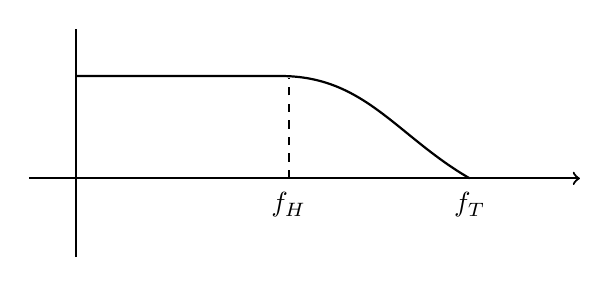
\begin{tikzpicture}[line width=0.8pt]
  \draw[->] (-0.6,0) -- (6.4,0);
  \draw (0,-1.0) -- (0,1.9);
  \draw (0,1.3) -- (2.6,1.3) to[out=0,in=150] (5.0,0);
  \draw[dashed] (2.7,0) -- (2.7,1.28);
  \node[below] at (2.7,-0.05) {$f_H$};
  \node[below] at (5.0,-0.05) {$f_T$};
\end{tikzpicture}
\end{center}

\end{document}
